%-----------------------------------------------------------------------------%
\chapter{\babEmpat}
%-----------------------------------------------------------------------------%
Bab ini menyajikan penjabaran mendalam mengenai realisasi teknis dari metodologi penelitian yang telah diuraikan pada Bab 3. Fokus utama adalah pada langkah-langkah konkret yang diambil untuk membangun lingkungan eksperimen, mengembangkan artefak perangkat lunak yang diuji, dan mengaplikasikan teknik \f{code virtualization} menggunakan platform VxLang. Pembahasan mencakup detail penyiapan lingkungan, arsitektur aplikasi studi kasus, implementasi \f{benchmark} performa, dan proses integrasi VxLang itu sendiri.

%-----------------------------------------------------------------------------%
\section{Penyiapan Lingkungan Pengembangan}
%-----------------------------------------------------------------------------%
Fondasi dari penelitian eksperimental ini adalah lingkungan pengembangan yang konsisten dan terdefinisi dengan baik. Hal ini krusial untuk memastikan reliabilitas dan reproduktifitas hasil. Komponen-komponen kunci yang dikonfigurasi adalah sebagai berikut:

\begin{itemize}
	\item \bo{Sistem Operasi:} Seluruh proses pengembangan, kompilasi, dan eksekusi pengujian dilakukan pada \bo{Microsoft Windows 11 (64-bit)}. Pemilihan Windows sebagai platform utama didasarkan pada target \f{executable} PE (Portable Executable) yang umum didukung oleh \f{tool} proteksi perangkat lunak seperti VxLang.
	\item \bo{Compiler:} \bo{Clang} (versi 19.1.3), diakses melalui antarmuka \bo{\code{clang-cl}}, dipilih sebagai \f{compiler} C++. Penggunaan \code{clang-cl} memastikan kompatibilitas biner dengan toolchain Microsoft Visual C++ (MSVC), yang seringkali menjadi prasyarat atau lingkungan yang didukung optimal oleh VxLang, sambil tetap memanfaatkan kemampuan analisis dan optimasi modern dari Clang. Proyek ini dikompilasi dengan standar bahasa \bo{C++17}.
	\item \bo{Build System \& Generator:} \bo{CMake} (versi 3.31) digunakan sebagai \f{meta-build system} untuk mengelola kompleksitas \f{build} lintas target dan dependensi. File \code{CMakeLists.txt} mendefinisikan target-target \f{build}, dependensi, dan opsi kompilasi. \bo{Ninja} (versi 1.12.1) digunakan sebagai \f{build generator} di bawah CMake untuk mempercepat proses kompilasi paralel. Konfigurasi \code{CMAKE\_EXPORT\_COMPILE\_COMMANDS} diaktifkan untuk memfasilitasi integrasi dengan \f{tool} analisis kode.
	\item \bo{Integrated Development Environment (IDE):} Neovim dengan LSP Clangd digunakan untuk efisiensi dalam penulisan kode, navigasi, dan \f{debugging} awal.
	\item \bo{Manajemen Dependensi \& Library Pihak Ketiga:} Library eksternal dikelola secara manual dengan menempatkan \f{header} di direktori \code{includes} dan \code{deps}, serta file library (\code{.lib}) di direktori \code{lib}. Library utama yang digunakan meliputi:
	      \begin{itemize}
		      \item \bo{VxLang SDK:} Terdiri dari file \f{header} (\code{includes/vxlang/vxlib.h}) yang mendefinisikan makro penanda virtualisasi (\code{VL\_VIRTUALIZATION\_BEGIN}, \code{VL\_VIRTUALIZATION\_END}) dan library statis (\code{lib/vxlib64.lib}) yang diperlukan oleh proses virtualisasi.
		      \item \bo{Qt Framework:} Versi \bo{6.\textit{x}} (MSVC 2022 64-bit) diintegrasikan menggunakan \code{find\_package(Qt6)} CMake. Modul \code{Widgets} digunakan untuk komponen GUI.
		      \item \bo{Dear ImGui:} Library Dear ImGui beserta \f{backend} \bo{GLFW} dan \bo{OpenGL3} di-\f{compile} sebagai bagian dari proyek (\code{deps/*.cpp}).
		      \item \bo{libcurl:} Digunakan untuk komunikasi HTTP pada aplikasi autentikasi varian \f{cloud}.
		      \item \bo{OpenSSL:} Versi \bo{3.\textit{x}} (\code{libssl}, \code{libcrypto}) digunakan untuk implementasi enkripsi AES pada \f{benchmark} performa.
		      \item \bo{nlohmann/json:} Library C++ \f{header-only} untuk menangani data JSON pada varian \f{cloud}.
	      \end{itemize}
\end{itemize}

%-----------------------------------------------------------------------------%
\section{Implementasi Pengujian Autentikasi}
%-----------------------------------------------------------------------------%
Bagian ini berfokus pada pengembangan aplikasi yang mensimulasikan proses login pengguna, yang kemudian menjadi subjek analisis \f{reverse engineering} sebelum dan sesudah penerapan VxLang. Pendekatan analisis mencakup analisis statis menggunakan Ghidra dan analisis dinamis menggunakan x64dbg, keduanya bertujuan mengidentifikasi dan mencoba mem-\textit{bypass} logika autentikasi.

Diagram alur persiapan \f{executable} disajikan pada Gambar \ref{fig:flow_auth_prep_rev}. Proses analisis statis dan dinamis, termasuk upaya \textit{bypass}, diilustrasikan pada Gambar \ref{fig:flow_auth_analysis_rev}. Proses ini melibatkan kompilasi kode sumber menjadi dua versi: versi asli (non-virtualized) dan versi \textit{intermediate} yang telah ditandai dengan makro VxLang dan ditautkan dengan pustaka VxLang (\texttt{vxlib64.lib}). Versi \textit{intermediate} ini kemudian diproses lebih lanjut menggunakan \textit{tool command-line} \texttt{vxlang.exe}. Konfigurasi lisensi vxlang ditangani melalui \textit{file} \texttt{vxlang.vxm} yang berada satu direktori dengan \textit{vxlang.exe}. Analisis dinamis dimulai dengan langkah serupa analisis statis, yaitu mencari \textit{string} atau pola kode yang relevan di dalam \textit{debugger} (x64dbg) untuk membantu menemukan lokasi logika autentikasi. Setelah lokasi potensial ditemukan, \textit{breakpoint} dipasang. Upaya \textit{bypass} kemudian dilakukan baik secara statis (mem-\textit{patch} file \textit{executable} menggunakan Ghidra) maupun secara dinamis (mem-\textit{patch} instruksi \textit{jump} kondisional atau memanipulasi register/memori secara langsung di x64dbg saat program berjalan).

%--- DIAGRAM PERSIAPAN AUTH ---
\begin{figure}[htbp]
	\centering
	% Menggunakan scale daripada resizebox
	\begin{tikzpicture}[
			scale=0.85, transform shape, % Skala diagram & teks
			node distance=3cm and 2.2cm, % Jarak antar node
			>=latex,
			block/.style={rectangle, draw, fill=blue!10, text width=9em, text centered, rounded corners, minimum height=3em},
			line/.style={draw, -latex'},
			io/.style={trapezium, trapezium left angle=70, trapezium right angle=110, draw, fill=orange!10, text centered, minimum height=2em}
		]
		% Nodes
		\node [block] (start) {Mulai};
		\node [block, below of=start, text width=10em] (prep_code) {Siapkan Kode Sumber Aplikasi (Console/Qt/ImGui)};
		\node [block, below left=1cm and 0.5cm of prep_code, text width=10em] (build_no_vm) {Build Tanpa VM (`cmake`, `ninja`)};
		\node [block, below right=1cm and 0.5cm of prep_code, text width=10em] (add_macro) {Tambah Makro VxLang (`VL\_...\_BEGIN/END`)};
		\node [block, below of=add_macro, text width=10em] (build_with_vm) {Build Dengan Penanda VM (`cmake -D...`, `ninja`)};
		\node [io, below of=build_with_vm, text width=10em] (vx_tool) {Proses dengan VxLang Tool (Input: JSON Config)};
		\node [block, below of=build_no_vm, yshift=-2cm] (exe_asli) {Executable Asli};
		\node [block, below of=vx_tool] (exe_vm) {Executable Virtualized};

		% Paths
		\path [line] (start) -- (prep_code);
		\path [line] (prep_code) |- (build_no_vm);
		\path [line] (prep_code) |- (add_macro);
		\path [line] (add_macro) -- (build_with_vm);
		\path [line] (build_with_vm) -- (vx_tool);
		\path [line] (build_no_vm) -- (exe_asli);
		\path [line] (vx_tool) -- (exe_vm);

		% Grouping Preparation
		\node [draw, dashed, inner sep=6pt, fit=(prep_code) (build_no_vm) (add_macro) (build_with_vm) (vx_tool) (exe_asli) (exe_vm)] {};
	\end{tikzpicture}
	\caption{Diagram Alur Persiapan Executable untuk Pengujian Autentikasi.}
	\label{fig:flow_auth_prep_rev} % Label SETELAH caption
\end{figure}
%--- AKHIR DIAGRAM PERSIAPAN AUTH ---

%--- DIAGRAM ANALISIS AUTH ---
\begin{figure}[htbp]
	\centering
	\begin{tikzpicture}[
			scale=0.8, transform shape,
			node distance=1.5cm and 1cm,
			>=latex,
			block/.style={rectangle, draw, fill=blue!10, text width=8em, text centered, rounded corners, minimum height=3em},
			proc/.style={rectangle, draw, fill=purple!10, text width=11em, text centered, rounded corners, minimum height=3em},
			test/.style={rectangle, draw, fill=orange!10, text width=10em, text centered, rounded corners, minimum height=3em},
			result/.style={ellipse, draw, fill=yellow!10, text centered, minimum height=3em, text width=15em},
			line/.style={draw, -latex'}
		]
		% Input Executables
		\node [block] (exe_asli) {Executable Asli};
		\node [block, right=8cm of exe_asli] (exe_vm) {Executable Virtualized};

		% Static Analysis / Patching Path
		\node [proc, below=1cm of exe_asli] (static_ghidra_asli) {Ghidra: Cari String, Identifikasi Logika/Jump Auth};
		\node [proc, below=1cm of exe_vm] (static_ghidra_vm) {Ghidra: Cari String (jika ada), Identifikasi Operasi VM};
		\node [proc, below=1cm of static_ghidra_asli] (static_patch_asli) {Ghidra: Patch Instruksi Jump Kondisional};
		\node [proc, below=1cm of static_ghidra_vm] (static_patch_vm) {Ghidra: Coba Patch Operasi VM (jika mungkin)};
		\node [test, below=1cm of static_patch_asli] (static_test_asli) {Uji Aplikasi Hasil Patch Statis};
		\node [test, below=1cm of static_patch_vm] (static_test_vm) {Uji Aplikasi Hasil Patch Statis};

		% Dynamic Analysis / Manipulation Path
		\node [proc, below=1cm of static_test_asli] (dynamic_x64_asli) {x64dbg: Run, Cari String, Breakpoint di Logika Auth};
		\node [proc, below=1cm of static_test_vm] (dynamic_x64_vm) {x64dbg: Run, Coba Cari String/Op VM, Breakpoint};
		\node [proc, below=1cm of dynamic_x64_asli] (dynamic_manip_asli) {x64dbg: Manipulasi Runtime (Patch Jump, Ubah Register/Memory)};
		\node [proc, below=1cm of dynamic_x64_vm] (dynamic_manip_vm) {x64dbg: Coba Manipulasi State VM};
		\node [test, below=1cm of dynamic_manip_asli] (dynamic_test_asli) {Uji Hasil Manipulasi/Patch Dinamis};
		\node [test, below=1cm of dynamic_manip_vm] (dynamic_test_vm) {Uji Hasil Manipulasi Dinamis};

		% Evaluation
		\node [result, below=2cm of $(dynamic_test_asli)!0.5!(dynamic_test_vm)$] (eval_result) {Evaluasi: Perbandingan Tingkat Kesulitan \& Keberhasilan Bypass (Asli vs VM, Statis vs Dinamis)};

		% Paths
		% Static
		\path [line] (exe_asli) -- (static_ghidra_asli);
		\path [line] (exe_vm) -- (static_ghidra_vm);
		\path [line] (static_ghidra_asli) -- (static_patch_asli);
		\path [line] (static_ghidra_vm) -- (static_patch_vm);
		\path [line] (static_patch_asli) -- (static_test_asli);
		\path [line] (static_patch_vm) -- (static_test_vm);
		% Dynamic
		\path [line] (static_test_asli) -- (dynamic_x64_asli);
		\path [line] (static_test_vm) -- (dynamic_x64_vm);
		\path [line] (dynamic_x64_asli) -- (dynamic_manip_asli);
		\path [line] (dynamic_x64_vm) -- (dynamic_manip_vm);
		\path [line] (dynamic_manip_asli) -- (dynamic_test_asli);
		\path [line] (dynamic_manip_vm) -- (dynamic_test_vm);
		% Evaluation
		\path [line] (dynamic_test_asli) |- (eval_result);
		\path [line] (dynamic_test_vm) |- (eval_result);

		% Optional Grouping
		\node [draw, dashed, inner sep=6pt, fit=(static_ghidra_asli)(static_patch_asli)(static_test_asli)(dynamic_x64_asli)(dynamic_manip_asli)(dynamic_test_asli)] {};
		\node [draw, dashed, inner sep=6pt, fit=(static_ghidra_vm)(static_patch_vm)(static_test_vm)(dynamic_x64_vm)(dynamic_manip_vm)(dynamic_test_vm)] {};

	\end{tikzpicture}
	\caption{Diagram Alur Analisis Upaya Bypass Autentikasi.}
	\label{fig:flow_auth_analysis_rev} % Label SETELAH caption
\end{figure}
%--- AKHIR DIAGRAM ANALISIS AUTH ---

\subsection{Aplikasi Studi Kasus Autentikasi}
Tiga jenis aplikasi dengan dua varian mekanisme autentikasi dikembangkan:

\begin{enumerate}
	\item \bo{Aplikasi Konsol (\code{console}, \code{console\_cloud}):} Aplikasi CLI sederhana.
	      \begin{itemize}
		      \item \bo{Varian Hardcoded (\code{src/console/console.cpp}):} Membandingkan input \code{std::cin} dengan \f{string} literal (\f{"seno"}, \f{"rahman"}) menggunakan \code{std::string::compare()}.
		            \begin{listing}[H] % Ganti cpp menjadi bahasa yang sesuai jika perlu
			            \begin{minted}{cpp}
// ... setelah input username & password ...
if (inputUsername.compare("seno") == 0 &&
    inputPassword.compare("rahman") == 0) {
  std::cout << "Authorized!" << std::endl;
} else {
  std::cout << "Not authorized." << std::endl;
}
// ...
                    \end{minted}
			            \caption{Logika Perbandingan Hardcoded (Konsol)}
			            \label{lst:console_hardcoded}
		            \end{listing}
		      \item \bo{Varian Cloud (\code{src/console/console\_cloud.cpp}):} Menggunakan \code{send\_login\_request} dari \code{includes/cloud.hpp} untuk mengirim kredensial via HTTP POST ke \code{http://localhost:9090/login}.
\begin{figure}[H]
	          \centering
	          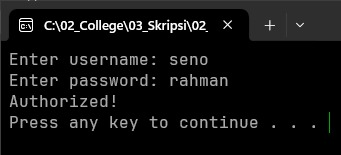
\includegraphics[height=0.25\textheight]{\Assets/console_app.jpeg} % Sesuaikan height/width jika perlu
	          \caption{Tampilan Aplikasi Autentikasi Varian Konsol saat dijalankan.}
	          \label{fig:console_app_ui}
	      \end{figure}
	      \end{itemize}
	\item \bo{Aplikasi Qt (\code{app\_qt}, \code{app\_qt\_cloud}):} Aplikasi GUI menggunakan Qt Widgets. UI dari \code{src/app\_qt/forms/todo\_auth.ui}.
	      \begin{itemize}
		      \item \bo{Varian Hardcoded (\code{src/app\_qt/src/todo\_auth.cpp}):} Logika serupa Kode \ref{lst:console_hardcoded} ditempatkan dalam \f{slot} \code{on\_button\_login\_clicked()}, menggunakan \code{ui->input\_User->text()} dan \code{ui->input\_Pass->text()}. Hasil via \code{QMessageBox}.
		      \item \bo{Varian Cloud (\code{src/app\_qt/src/todo\_auth\_cloud.cpp}):} Slot memanggil \code{send\_login\_request}.
	      \end{itemize}
        \begin{figure}[H]
	          \centering
	          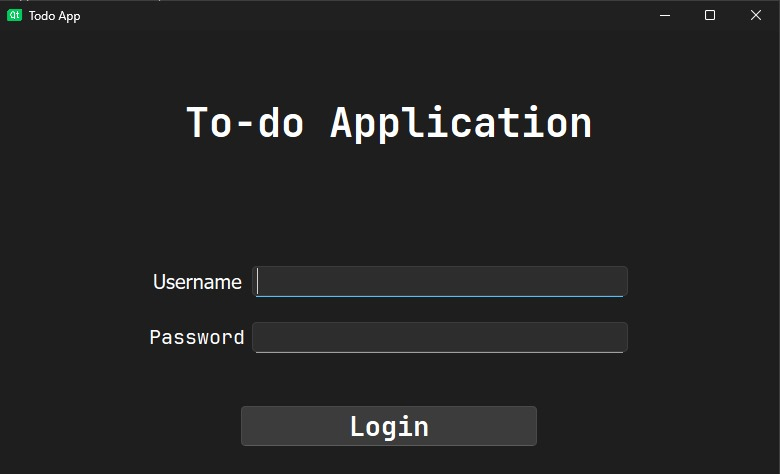
\includegraphics[height=0.3\textheight]{\Assets/qt_app.jpeg} % Sesuaikan height/width jika perlu
	          \caption{Tampilan Antarmuka Aplikasi Autentikasi Varian Qt.}
	          \label{fig:qt_app_ui}
	      \end{figure}
	\item \bo{Aplikasi Dear ImGui (\code{app\_imgui}, \code{app\_imgui\_cloud}):} Aplikasi GUI \f{immediate mode} menggunakan Dear ImGui, GLFW, OpenGL.
	      \begin{itemize}
		      \item \bo{Varian Hardcoded (\code{src/app\_imgui/login.cpp}):} Logika perbandingan dalam \code{Login::LoginWindow} saat \code{ImGui::Button("Login")} ditekan. Hasil ditampilkan via \code{MessageBoxW}.
		      \item \bo{Varian Cloud (\code{src/app\_imgui/login\_cloud.cpp}):} Memanggil \code{send\_login\_request} saat tombol login ditekan, menampilkan hasil via \code{MessageBoxW}.
	      \end{itemize}
        \begin{figure}[H]
	          \centering
	          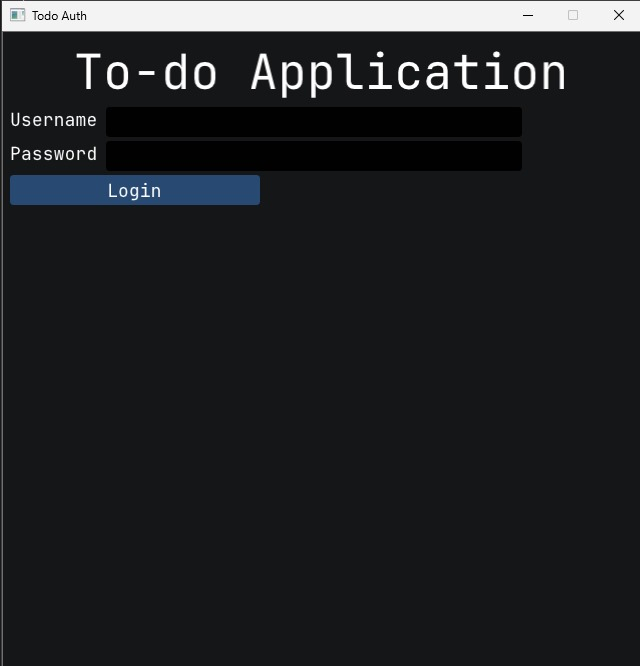
\includegraphics[height=0.5\textheight]{\Assets/imgui_app.jpeg} % Sesuaikan height/width jika perlu
	          \caption{Tampilan Antarmuka Aplikasi Autentikasi Varian Dear ImGui.}
	          \label{fig:imgui_app_ui}
	      \end{figure}
\end{enumerate}

\bo{Implementasi Fungsi Permintaan Cloud (\code{cloud.hpp}):}
Fungsi \code{send\_login\_request} bertanggung jawab untuk mengemas kredensial ke dalam format JSON dan mengirimkannya ke server \textit{backend} menggunakan library \code{libcurl}. Snippet berikut menyoroti langkah-langkah utamanya:
\begin{listing}[H]
	\begin{minted}{cpp}
// Potongan dari includes/cloud.hpp
bool send_login_request(const std::string &username,
const std::string &password, HWND /window/ = NULL) {
  CURL *curl;
  CURLcode res;
  std::string readBuffer;
  std::string url = "http://localhost:9090/login";
  
  // 1. Buat payload JSON
  nlohmann::json payload;
  payload["username"] = username;
  payload["password"] = password;
  std::string jsonStr = payload.dump();
  
  curl = curl_easy_init();
  if (curl) {
    struct curl_slist *headers = nullptr;
    headers = curl_slist_append(headers, "Content-Type: application/json");
    
    // 2. Konfigurasi request cURL (URL, Headers, Body, Callback, Timeout)
    curl_easy_setopt(curl, CURLOPT_URL, url.c_str());
    curl_easy_setopt(curl, CURLOPT_HTTPHEADER, headers);
    curl_easy_setopt(curl, CURLOPT_POSTFIELDS, jsonStr.c_str());
    curl_easy_setopt(curl, CURLOPT_WRITEFUNCTION, WriteCallback);
    curl_easy_setopt(curl, CURLOPT_WRITEDATA, &readBuffer);
    curl_easy_setopt(curl, CURLOPT_TIMEOUT, 5L); // Timeout 5 detik
    
    // 3. Kirim request
    res = curl_easy_perform(curl);
    
    // 4. Cleanup cURL
    curl_easy_cleanup(curl);
    curl_slist_free_all(headers);
    
    // 5. Handle error cURL
    if (res != CURLE_OK || readBuffer.empty()) {
       // Error handling (misal: log error)
       return false;
    }
  }
  return false; // Gagal inisialisasi cURL
}
    \end{minted}
	\caption{Implementasi Fungsi \code{send\_login\_request}}
	\label{lst:send_login_request}
\end{listing}

\subsection{Implementasi Sisi Server (Varian Cloud)}
\f{Backend} API lokal untuk varian \f{cloud} diimplementasikan sebagai berikut:

\begin{itemize}
	\item \bo{Teknologi:} Go (Golang) untuk API (\code{server/backend/main.go}), PostgreSQL 15 untuk database, Docker dan Docker Compose untuk \f{deployment} (\code{server/docker-compose.yml}).
	\item \bo{API Endpoint \code{/login} (POST):} Menerima JSON, mengambil \f{salt/hash} dari DB, menghitung ulang \f{hash} input menggunakan PBKDF2-SHA256 (100k iterasi), membandingkan \f{hash} (\f{constant time}), mengembalikan \code{{"success": true/false}}.
	\item \bo{API Endpoint \code{/register} (POST):} Menerima JSON, generate \f{salt}, hitung \f{hash} PBKDF2, simpan ke DB.
	\item \bo{Database Schema (\code{server/postgres/init.sql}):} Tabel \code{users(username, password\_hash, salt)}. Menyisipkan user \f{default} (\f{seno}/rahman) dengan \f{hash/salt} precomputed.
\end{itemize}

%-----------------------------------------------------------------------------%
\section{Implementasi Pengujian Performa}
%-----------------------------------------------------------------------------%
Diagram alur untuk persiapan dan pelaksanaan pengujian performa diilustrasikan pada Gambar \ref{fig:flow_perf_rev}. Serupa dengan persiapan \textit{executable} untuk studi kasus autentikasi, artefak untuk \textit{benchmark} performa juga disiapkan dalam dua versi: asli dan \textit{intermediate} yang ditandai VxLang. \textit{Executable intermediate} tersebut kemudian diproses oleh \textit{tool command-line} \texttt{vxlang.exe} untuk menghasilkan versi tervirtualisasi akhir yang diuji.

%--- DIAGRAM PERF ---

\begin{figure}[htbp]
	\centering
	\begin{tikzpicture}[
			scale=0.8, transform shape, % <<-- Skala lebih kecil
			node distance=3cm and 1.5cm, % <<-- Kurangi jarak horizontal
			>=latex,
			block/.style={rectangle, draw, fill=blue!10, text width=8em, text centered, rounded corners, minimum height=3em},
			proc/.style={rectangle, draw, fill=purple!10, text width=10em, text centered, rounded corners, minimum height=3em},
			result/.style={ellipse, draw, fill=yellow!10, text centered, minimum height=3em},
			io/.style={trapezium, trapezium left angle=70, trapezium right angle=110, draw, fill=orange!10, text centered, minimum height=2em},
			line/.style={draw, -latex'}
		]
		% Nodes
		\node [block] (start) {Mulai};
		\node [block, below of=start, text width=10em] (prep_code) {Siapkan Kode Benchmark (QuickSort/AES/Size)};
		% Kolom Kiri (Asli)
		\node [block, below left=1cm and 0.3cm of prep_code, text width=10em] (build_no_vm) {Build Tanpa VM (`cmake`, `ninja`)}; % Geser lebih dekat
		\node [block, below of=build_no_vm, yshift=-1cm] (exe_asli) {Executable Asli}; % Sesuaikan posisi vertikal jika perlu
		\node [proc, below of=exe_asli, yshift=-0.5cm] (run_bench_asli) {Jalankan Benchmark Asli (Variasi Input/Ukuran)};
		\node [io, below of=run_bench_asli] (measure_asli) {Ukur Waktu/Ukuran};

		% Kolom Kanan (VM)
		\node [block, below right=1cm and 0.3cm of prep_code, text width=10em] (add_macro) {Tambah Makro VxLang (`VL\_...\_BEGIN/END`)}; % Geser lebih dekat
		\node [block, below of=add_macro, text width=10em] (build_with_vm) {Build Dengan Penanda VM (`cmake -D...`, `ninja`)};
		\node [io, below of=build_with_vm, text width=10em] (vx_tool) {Proses dengan VxLang Tool (Input: JSON Config)};
		\node [block, below of=vx_tool] (exe_vm) {Executable Virtualized};
		\node [proc, below of=exe_vm, yshift=-0.5cm] (run_bench_vm) {Jalankan Benchmark VM (Variasi Input/Ukuran)};
		\node [io, below of=run_bench_vm] (measure_vm) {Ukur Waktu/Ukuran};

		% Nodes Tengah Bawah
		\node [result, below=3.5cm of $(measure_asli)!0.5!(measure_vm)$] (analyze_data) {Analisis Data (Rata-rata, StdDev, Perbandingan)}; % Geser ke tengah
		\node [result, below=1.5cm of analyze_data] (eval_overhead) {Evaluasi Overhead Performa \& Trade-off};

		% Paths
		\path [line] (start) -- (prep_code);
		\path [line] (prep_code) |- (build_no_vm);
		\path [line] (prep_code) |- (add_macro);
		\path [line] (add_macro) -- (build_with_vm);
		\path [line] (build_with_vm) -- (vx_tool);
		\path [line] (build_no_vm) -- (exe_asli);
		\path [line] (vx_tool) -- (exe_vm);

		\path [line] (exe_asli) -- (run_bench_asli);
		\path [line] (exe_vm) -- (run_bench_vm);
		\path [line] (run_bench_asli) -- (measure_asli);
		\path [line] (run_bench_vm) -- (measure_vm);
		\path [line] (measure_asli) -- (analyze_data);
		\path [line] (measure_vm) -- (analyze_data);
		\path [line] (analyze_data) -- (eval_overhead);

		% Grouping (Optional) - Mungkin hapus jika terlalu lebar
		% \node [draw, dashed, inner sep=6pt, fit=(prep_code) (build_no_vm) (add_macro) (build_with_vm) (vx_tool) (exe_asli) (exe_vm)] {};
		% \node [draw, dashed, inner sep=6pt, fit=(run_bench_asli) (run_bench_vm) (measure_asli) (measure_vm) (analyze_data) (eval_overhead)] {};
	\end{tikzpicture}
	\caption{Diagram Alur Persiapan dan Pengujian Performa.}
	\label{fig:flow_perf_rev} % Label SETELAH caption
\end{figure}

%--- AKHIR DIAGRAM PERF ---

\subsection{Benchmark Algoritma Quick Sort (\code{QuickSort})}
\begin{itemize}
	\item \bo{Implementasi (\code{src/performance/quick\_sort.cpp}):} Menggunakan \code{std::vector<int>}, fungsi rekursif \code{quickSort}, dan \code{partition}.
	\item \bo{Data:} Vektor acak (1-1.000.000) ukuran bervariasi (100 s/d 3.000.000 elemen).
	\item \bo{Pengukuran:} \code{std::chrono::high\_resolution\_clock} mengukur waktu eksekusi \code{quickSort}. Diulang 100 kali per ukuran data. Rata-rata dan standar deviasi dihitung.
	\item \bo{Integrasi VxLang:} \code{VL\_VIRTUALIZATION\_BEGIN/END} membungkus \textit{seluruh isi} fungsi rekursif \code{quickSort}.

	      \begin{listing}[H]
		      \begin{minted}{cpp}
// Potongan dari src/performance/quick_sort.cpp
std::pair<double, double> measureSortingTime(size_t size, int runs = 10) {
  std::vector<double> times;
  for (int i = 0; i < runs; ++i) {
    std::vector<int> data = generateRandomVector(size);
    auto start = std::chrono::high_resolution_clock::now();
    quickSort(data, 0, data.size() - 1); // Fungsi yang divirtualisasi
    auto stop = std::chrono::high_resolution_clock::now();
    std::chrono::duration<double, std::milli> duration = stop - start;
    times.push_back(duration.count());
  }
  // ... (Calculate average and stdDev) ...
  return {average, stdDev};
}
        \end{minted}
		      \caption{Pengukuran Waktu Eksekusi QuickSort}
		      \label{lst:quicksort_measure}
	      \end{listing}
\end{itemize}

\subsection{Benchmark Enkripsi AES-CBC-256 (\code{Encryption})}
\begin{itemize}
	\item \bo{Implementasi:} Kelas \code{AESCipher} (\code{aes.h}, \code{aes.cpp}) menggunakan API \code{EVP} OpenSSL untuk AES-256-CBC.
	\item \bo{Data:} 1 GB data acak (1 juta blok @ 1024 byte), diproses per \f{batch} (misal, 10.000 blok/batch).
	\item \bo{Pengukuran:} \code{chrono} mengukur total waktu enkripsi/dekripsi seluruh \f{batch}. \f{Throughput} (MB/s) dihitung.
	\item \bo{Integrasi VxLang:} \code{VL\_VIRTUALIZATION\_BEGIN/END} membungkus \f{looping} pemanggilan \code{aes.encrypt()}/\code{decrypt()} di dalam fungsi \code{measureBatch...Time}.
\end{itemize}

\subsection{Pengukuran Ukuran File}
\begin{itemize}
	\item \bo{Implementasi:} Ukuran file \f{executable} diukur menggunakan fungsi \code{std::filesystem::file\_size} atau melalui \f{file explorer} Windows. Aplikasi \code{Size} (\code{src/performance/size.cpp}) dibuat khusus dengan data \textit{dummy} tersemat (\code{dummy.bin} via \code{dummy.rc}) untuk mensimulasikan aplikasi dengan aset data internal yang besar.
	\item \bo{Target Pengukuran:} Pengukuran ukuran file dilakukan pada \textbf{semua} target \f{executable} yang dihasilkan, baik versi asli maupun versi \textit{virtualized} (\code{*\_vm.exe}), termasuk \code{QuickSort}, \code{Encryption}, \code{Size}, \code{console}, \code{app\_imgui}, dan \code{app\_qt}, sesuai data pada Tabel \ref{tab:file_size}.
	\item \bo{Integrasi VxLang pada Target \code{Size}:} Makro \code{VL\_VIRTUALIZATION\_BEGIN/END} tetap disertakan dalam \code{main} pada target \code{Size} untuk memastikan \f{runtime} VxLang disertakan pada versi \code{size\_vm.exe}, sehingga memungkinkan perbandingan ukuran yang fokus pada \textit{overhead} \textit{runtime} itu sendiri.
\end{itemize}


\subsection{Integrasi dan Proses Virtualisasi VxLang}
Penerapan VxLang \bo{dilakukan} dengan langkah-langkah berikut:

\begin{enumerate}
	\item \bo{Penempatan Makro:} Makro \code{VL\_VIRTUALIZATION\_BEGIN/END} \bo{ditempatkan} membungkus logika autentikasi inti, fungsi rekursif \code{quickSort}, loop enkripsi/dekripsi, dan blok dummy di \code{Size}. Contoh penempatan pada aplikasi konsol hardcoded:
	      \begin{listing}[H]
		      \begin{minted}{cpp}
// ... (Input username/password) ...
VL_VIRTUALIZATION_BEGIN; // <-- Makro Awal

if (inputUsername.compare("seno") == 0 &&
    inputPassword.compare("rahman") == 0) {
  // ... (Authorized code) ...
} else {
  // ... (Not authorized code) ...
}

VL_VIRTUALIZATION_END; // <-- Makro Akhir
// ...
            \end{minted}
		      \caption{Penempatan Makro VxLang pada Logika Autentikasi}
          \end{listing}
\item \bo{Konfigurasi Build CMake:} File \texttt{CMakeLists.txt} memegang peranan sentral dalam mengelola proses kompilasi untuk menghasilkan kedua jenis \textit{executable}: asli (non-virtualized) dan \textit{intermediate} (\texttt{*\_vm.exe}) yang siap diproses oleh VxLang. Konfigurasi ini mencakup:
      \begin{itemize}
        \item Definisi \textit{preprocessor} \texttt{USE\_VL\_MACRO}: Opsi ini, biasanya dikontrol melalui \textit{flag} CMake (misalnya, \texttt{-DUSE\_VL\_MACRO=1}), digunakan untuk mengaktifkan makro-makro VxLang (\texttt{VL\_VIRTUALIZATION\_BEGIN}, dll.) yang didefinisikan dalam \texttt{includes/vxlang/vxlib.h}. Jika \texttt{USE\_VL\_MACRO} tidak didefinisikan, makro-makro tersebut menjadi kosong sehingga tidak ada kode VxLang yang aktif.
        \item Penautan Pustaka VxLang: Untuk \textit{build intermediate} (\texttt{*\_vm.exe}), pustaka statis VxLang (\texttt{vxlib64.lib}) perlu ditautkan. Pustaka ini berisi fungsi-fungsi yang dipanggil oleh makro VxLang saat \texttt{USE\_VL\_MACRO} aktif.
        \item Penamaan Output: \textit{Build system} dikonfigurasi untuk menghasilkan nama \textit{file output} yang berbeda untuk versi asli dan versi \textit{intermediate}, misalnya \texttt{nama\_target.exe} untuk versi asli dan \texttt{nama\_target\_vm.exe} untuk versi \textit{intermediate}.
      \end{itemize}
Sebagai ilustrasi, berikut adalah contoh penyederhanaan logika yang dapat ditemukan dalam \texttt{CMakeLists.txt} (fungsi \texttt{add\_project\_executables} pada proyek ini mengimplementasikan logika serupa secara lebih komprehensif):

\begin{listing}[H]
\begin{minted}[fontsize=\small]{cmake}
# Contoh logika CMake untuk target 'console'
# (Versi sederhana untuk ilustrasi)

# Target Asli (Non-VM)
add_executable(console src/console/console.cpp ...)
set_target_properties(console PROPERTIES OUTPUT_NAME "console")
# ... (tidak ada USE_VL_MACRO, tidak ada link ke vxlib64)

# Target Intermediate (untuk VxLang)
add_executable(console_vm_cmake_example src/console/console.cpp ...)
target_compile_definitions(console_vm_cmake_example PRIVATE USE_VL_MACRO)
target_link_libraries(console_vm_cmake_example PRIVATE vxlib64)
set_target_properties(console_vm_cmake_example PROPERTIES OUTPUT_NAME "console_vm")
\end{minted}
\captionof{listing}{Contoh Ilustratif Konfigurasi CMake untuk Build Asli dan Intermediate VxLang}
\label{lst:cmake_vxlang_integration_bab4}
\end{listing}

\item \bo{Proses Kompilasi dan Virtualisasi Aktual:} Proses keseluruhan untuk menghasilkan \textit{executable} tervirtualisasi melibatkan langkah-langkah berikut, yang diorkestrasi oleh kombinasi CMake, Ninja, dan skrip \texttt{virtualize.bat}:
    \begin{itemize}
        \item \textbf{Build Asli:} Jalankan perintah CMake (misalnya, \texttt{cmake -G Ninja -B build\_asli ..}) diikuti dengan perintah Ninja (\texttt{ninja -C build\_asli}). Proses ini akan menghasilkan \textit{executable} asli tanpa modifikasi VxLang di direktori \textit{output} yang ditentukan (misalnya, \texttt{build\_asli/bin/}).
        \item \textbf{Build Intermediate (\texttt{*\_vm.exe}):} Jalankan perintah CMake dengan \textit{flag} untuk mengaktifkan VxLang (misalnya, \texttt{cmake -G Ninja -B build\_vm -DUSE\_VL\_MACRO=1 ..}) diikuti dengan perintah Ninja (\texttt{ninja -C build\_vm}). Proses ini menghasilkan \textit{executable intermediate} (misalnya, \texttt{console\_vm.exe}) di direktori \textit{output} yang sesuai. \textit{Executable} ini sudah mengandung penanda VxLang dari makro dan tertaut dengan \texttt{vxlib64.lib}.
        \item \textbf{Proses Virtualisasi VxLang (\texttt{*\_vxm.exe}):} \textit{Executable intermediate} (\texttt{*\_vm.exe}) kemudian diproses menggunakan \textit{tool command-line} \texttt{vxlang.exe}. Skrip \texttt{virtualize.bat} dalam proyek ini mengotomatiskan langkah ini untuk semua target yang relevan. Contoh baris perintah yang mungkin dijalankan oleh skrip ini untuk target \texttt{console\_vm.exe} adalah:
            \begin{listing}[H]
            \begin{minted}[fontsize=\small]{batch}
            REM Contoh dari virtualize.bat (disesuaikan untuk kejelasan)
            set "vxlang_tool_path=vxlang\vxlang.exe"
            set "intermediate_exe_path=bin\console\Release\console_vm.exe"
            
            REM Perintah aktual untuk menjalankan virtualisasi
            %vxlang_tool_path% %intermediate_exe_path%
            \end{minted}
            \captionof{listing}{Contoh Baris Perintah dari Skrip untuk Menjalankan VxLang Tool}
            \label{lst:virtualize_bat_example_bab4}
            \end{listing}
        Pemanggilan \texttt{vxlang.exe} pada \texttt{console\_vm.exe} akan menganalisis penanda virtualisasi, mengganti kode \textit{native} yang ditandai dengan representasi \textit{bytecode} internal, dan menyematkan \textit{runtime Virtual Machine} (VM) yang diperlukan. Proses ini secara otomatis menghasilkan \textit{file executable} akhir yang telah tervirtualisasi dengan nama yang dimodifikasi, yaitu \texttt{console\_vm.vxm.exe}, yang disimpan di direktori yang sama dengan \textit{file input}-nya. \textit{Executable} \texttt{*\_vxm.exe} inilah yang kemudian menjadi subjek utama pengujian keamanan dan analisis dampak performa dalam penelitian ini.
    \end{itemize}
\end{enumerate}

%-----------------------------------------------------------------------------%
\section{Studi Kasus: Aplikasi Potensial Berbahaya dan Malware}
\label{sec:implementasi_lilith_dan_malware} 
%-----------------------------------------------------------------------------%
Selain aplikasi studi kasus autentikasi dan \textit{benchmark} performa yang dikembangkan secara khusus, penelitian ini juga melibatkan analisis terhadap aplikasi \textit{Remote Administration Tool} (RAT) \textit{open-source} bernama Lilith. Penggunaan Lilith bertujuan untuk menguji efektivitas dan dampak VxLang pada perangkat lunak yang lebih kompleks dan memiliki karakteristik yang sering diasosiasikan dengan \textit{malware} atau \textit{Potentially Unwanted Application} (PUA).

\subsection{Deskripsi Singkat Lilith RAT}
Lilith adalah sebuah RAT yang dikembangkan menggunakan C++ dan dirancang untuk platform Windows. Kode sumbernya tersedia secara publik \cite{LilithRAT}, memungkinkan untuk kompilasi dan modifikasi. Fungsionalitas utama yang ditawarkan oleh Lilith mencakup kemampuan untuk:
\begin{itemize}
    \item Membuat koneksi terbalik (\textit{reverse connection}) dari klien ke server.
    \item Mengeksekusi perintah pada sistem klien secara jarak jauh melalui antarmuka \textit{command-line}.
    \item Melakukan \textit{keylogging} untuk merekam ketikan papan ketik pada mesin klien.
    \item Menyediakan mekanisme persistensi sederhana.
    \item Mentransfer berkas antara server dan klien (fungsionalitas ini ada dalam kode sumbernya, meskipun mungkin tidak menjadi fokus utama pengujian virtualisasi dalam penelitian ini).
\end{itemize}
Karena fungsionalitas tersebut, Lilith RAT menjadi objek studi yang menarik untuk melihat bagaimana virtualisasi kode dapat mempersulit analisis terhadap perangkat lunak dengan potensi penggunaan ganda (\textit{dual-use}).

\subsection{Persiapan \textit{Executable} Lilith untuk Analisis}
Proses persiapan \textit{executable} klien Lilith untuk analisis virtualisasi mengikuti langkah-langkah serupa dengan aplikasi studi kasus lainnya, dengan penekanan pada identifikasi dan penandaan bagian kode yang kritikal.

\begin{enumerate}
    \item \bo{Akuisisi dan Kompilasi Kode Sumber Asli:} Kode sumber Lilith RAT (khususnya komponen klien) diunduh dari repositori publiknya. Kompilasi dilakukan menggunakan lingkungan pengembangan yang telah disiapkan (Clang/clang-cl, CMake, Ninja dengan standar C++17) untuk menghasilkan \textit{executable} klien Lilith versi asli (\texttt{Lilith\_Client.exe}). Komponen server Lilith juga dikompilasi dalam versi aslinya dan digunakan untuk menguji fungsionalitas klien.

    \item \bo{Identifikasi dan Penandaan Kode Kritis dengan Makro VxLang:}
    Mengingat kompleksitas Lilith, virtualisasi tidak diterapkan pada keseluruhan kode sumber klien. Sebaliknya, fokus diberikan pada fungsi-fungsi dan blok-blok kode yang dianggap paling krusial untuk operasional RAT dan yang paling mungkin menjadi target analisis oleh \textit{reverse engineer}. Makro \texttt{VL\_VIRTUALIZATION\_BEGIN} dan \texttt{VL\_VIRTUALIZATION\_END} dari VxLang SDK disisipkan secara strategis untuk membungkus bagian-bagian berikut dalam kode sumber klien Lilith (\texttt{src/Lilith/client/}):
    \begin{itemize}
        \item \textbf{Pemrosesan Perintah Inti:} Dalam fungsi seperti \texttt{Client::ProcessPacketType} (pada berkas \texttt{client.cpp}), logika yang menangani paket instruksi dari server dan memanggil fungsi \texttt{General::processCommand} divirtualisasi. Bagian yang memproses perintah CMD jarak jauh melalui objek \texttt{CMD::cmdptr} juga ditandai. Contoh penempatan makro secara ilustratif dapat dilihat pada Lampiran \ref{app:lilith_vxlang_macros_full} (Kode \ref{lst:lilith_vxlang_macros_appendix_full}).
        \item \textbf{Inisialisasi dan Koneksi:} Bagian kode dalam konstruktor \texttt{Client::Client} atau fungsi \texttt{Client::Connect} yang bertanggung jawab untuk inisialisasi koneksi jaringan ke server juga dipertimbangkan untuk virtualisasi untuk mengaburkan detail mekanisme koneksi.
        \item \textbf{Loop Utama Pemrosesan Paket:} Loop utama dalam \texttt{Client::ClientThread} yang terus menerus menerima dan memproses paket dari server menjadi target virtualisasi untuk mempersulit pemahaman alur kerja komunikasi.
        \item \textbf{Fungsi Sensitif Tambahan:} Beberapa fungsi pendukung dalam \texttt{general.cpp} atau \texttt{cmdRedirect.cpp} yang terkait langsung dengan eksekusi perintah atau interaksi sistem juga ditandai, jika relevan.
    \end{itemize}
    Penempatan makro dilakukan dengan hati-hati untuk memastikan fungsionalitas utama tetap terjaga sambil memaksimalkan kesulitan analisis.

    \item \bo{Build \textit{Executable Intermediate} (\texttt{Lilith\_Client\_vm.exe}):}
    Setelah penandaan kode, klien Lilith dikompilasi ulang dengan mengaktifkan \textit{flag preprocessor} \texttt{USE\_VL\_MACRO} melalui konfigurasi CMake. \textit{Executable} yang dihasilkan (\texttt{Lilith\_Client\_vm.exe}) secara otomatis tertaut dengan pustaka VxLang (\texttt{vxlib64.lib}).

    \item \bo{Proses Virtualisasi Akhir dengan VxLang Tool:}
    \textit{Executable intermediate} \texttt{Lilith\_Client\_vm.exe} kemudian diproses menggunakan \textit{tool command-line} \texttt{vxlang.exe}. Proses ini diotomatisasi melalui skrip \texttt{virtualize.bat}, yang menjalankan perintah serupa dengan:
    \begin{listing}[H]
    \begin{minted}[fontsize=\small]{batch}
REM Contoh dari virtualize.bat untuk Lilith Client
set "vxlang_tool_path=vxlang\vxlang.exe"
set "lilith_intermediate_path=bin\Lilith_Client\Release\Lilith_Client_vm.exe"
%vxlang_tool_path% %lilith_intermediate_path%
    \end{minted}
    \captionof{listing}{Perintah Virtualisasi untuk Klien Lilith RAT} % Label diubah agar unik
    \label{lst:virtualize_lilith_example_bab4_revised}
    \end{listing}
    Perintah ini menghasilkan \textit{executable} klien Lilith yang telah tervirtualisasi sepenuhnya, yaitu \texttt{Lilith\_Client\_vm.vxm.exe}. Berkas inilah yang kemudian digunakan untuk pengujian fungsionalitas, analisis keamanan statis/dinamis, dan pengujian deteksi VirusTotal yang hasilnya dipaparkan pada Bab \ref{bab:hasil_penelitian_lilith}.
\end{enumerate}

Persiapan yang cermat ini memastikan bahwa kedua versi klien Lilith (asli dan tervirtualisasi) dapat dibandingkan secara adil untuk mengevaluasi dampak VxLang.

\subsection{Tantangan dalam Penempatan Makro VxLang pada Lilith RAT}
\label{subsec:tantangan_makro_lilith}
Proses penerapan makro virtualisasi VxLang pada kode sumber klien Lilith RAT mengungkapkan sebuah aspek krusial, yaitu sensitivitas fungsionalitas program terhadap penempatan makro yang kurang tepat. Meskipun tujuan utama virtualisasi adalah untuk melindungi bagian kode yang paling kritikal, pengalaman dalam studi kasus ini menunjukkan bahwa tidak semua blok kode dapat divirtualisasi secara langsung tanpa menimbulkan efek samping yang merugikan.

Sebagai contoh, upaya awal untuk memvirtualisasi blok kode yang lebih besar atau yang memiliki interaksi kompleks dengan alur kontrol dan pemanggilan fungsi eksternal pada Lilith RAT menemui kendala. Salah satu observasi spesifik terjadi pada penanganan paket \texttt{PacketType::CMDCommand} dalam fungsi \texttt{Client::ProcessPacketType}. Ketika seluruh blok \texttt{case} untuk \texttt{CMDCommand} dibungkus dengan makro \texttt{VL\_VIRTUALIZATION\_BEGIN} dan \texttt{VL\_VIRTUALIZATION\_END}, seperti pada ilustrasi berikut:

\begin{listing}[H]
\begin{minted}[fontsize=\small]{cpp}
// Ilustrasi penempatan makro yang awalnya menyebabkan masalah
case PacketType::CMDCommand: {
    VL_VIRTUALIZATION_BEGIN; //<- Awalnya di sini
    std::string msg;
    if (!GetString(msg)) // Fungsi untuk mendapatkan string dari jaringan
      return false;

    if (CMD::cmdptr != NULL) {
      CMD::cmdptr->writeCMD(msg); // Fungsi untuk menulis perintah ke CMD
    } else {
      SendString("Initiate a CMD session first.", PacketType::Warning);
    }
    VL_VIRTUALIZATION_END; //<- Awalnya di sini
    break;
}
\end{minted}
\captionof{listing}{Contoh Ilustratif Penempatan Awal Makro VxLang pada Lilith RAT yang Menimbulkan Masalah Fungsionalitas}
\label{lst:lilith_macro_problem_cmd}
\end{listing}

Penempatan makro seperti pada Kode \ref{lst:lilith_macro_problem_cmd} menyebabkan aplikasi klien Lilith mengalami \textit{crash} atau \textit{hang} ketika server mengirimkan perintah yang berkaitan dengan \texttt{PacketType::CMDCommand}. Fungsionalitas baru dapat dipulihkan ketika virtualisasi diterapkan secara lebih granular, misalnya dengan memindahkan makro untuk hanya membungkus pemanggilan fungsi spesifik di dalam logika tersebut, seperti di dalam fungsi \texttt{CMD::cmdptr->writeCMD(msg)} itu sendiri, bukan seluruh blok \texttt{case}.

Kendala serupa juga ditemui pada bagian kode yang bertanggung jawab untuk mengirimkan respons perintah kembali ke server:
\begin{listing}[H]
\begin{minted}[fontsize=\small]{cpp}
// Ilustrasi penempatan makro lain yang menyebabkan masalah
 
VL_VIRTUALIZATION_BEGIN; //<- Penempatan ini menyebabkan hang/crash
SendString(General::processCommand(msg), PacketType::Instruction);
VL_VIRTUALIZATION_END;

\end{minted}
\captionof{listing}{Contoh Ilustratif Penempatan Makro VxLang Lain yang Menimbulkan Masalah}
\label{lst:lilith_macro_problem_send}
\end{listing}
Ketika pemanggilan fungsi \texttt{SendString} (yang melibatkan operasi jaringan) bersama dengan \texttt{General::processCommand} divirtualisasi seperti pada Kode \ref{lst:lilith_macro_problem_send}, klien Lilith akan mengalami \textit{crash} dan terputus dari server saat server mencoba mengaktifkan fitur seperti \texttt{remoteControl cmd}.

Temuan ini mengindikasikan bahwa \textit{tool} virtualisasi seperti VxLang mungkin memiliki interaksi yang kompleks dengan struktur kode tertentu, terutama yang melibatkan alur kontrol non-linear (seperti \texttt{switch-case}), operasi I/O, atau pemanggilan fungsi yang mengubah konteks eksekusi secara signifikan. Oleh karena itu, keberhasilan implementasi VxLang tidak hanya bergantung pada identifikasi bagian kode yang sensitif, tetapi juga pada eksperimen dan pengujian fungsional yang cermat untuk memastikan bahwa penempatan makro virtualisasi tidak merusak integritas operasional aplikasi. Hal ini menekankan pentingnya pendekatan virtualisasi yang selektif dan teruji.

\subsection{Persiapan Sampel Malware Tambahan untuk Analisis VirusTotal}
\label{subsec:persiapan_malware_tambahan}
Selain Lilith RAT, penelitian ini melibatkan analisis dampak virtualisasi VxLang terhadap deteksi oleh VirusTotal untuk sembilan sampel \textit{malware} atau \textit{Potentially Unwanted Application} (PUA) tambahan. Sampel-sampel ini, yang diperoleh dari berbagai sumber repositori publik atau koleksi sampel analisis, adalah: \textit{Al-Khaser, donut, DripLoader, FilelessPELoader, JuicyPotato, ParadoxiaClient, PELoader, RunPE-In-Memory,} dan \textit{SigLoader}.

Untuk setiap sampel \textit{malware/PUA} tersebut, dua versi \textit{executable} disiapkan untuk perbandingan di VirusTotal:
\begin{enumerate}
    \item \textbf{Versi Asli (Non-Virtualized):} Ini adalah berkas \textit{executable} asli dari sampel \textit{malware/PUA} yang bersangkutan, tanpa modifikasi atau pemrosesan lebih lanjut oleh VxLang.
    \item \textbf{Versi Virtualized (VM):} Berkas \textit{executable} asli dari setiap sampel \textit{malware/PUA} kemudian diproses menggunakan \textit{tool command-line} \texttt{vxlang.exe}. Mengingat sifat \textit{closed-source} dari sebagian besar sampel ini dan tidak adanya kode sumber untuk penempatan makro SDK secara manual, proses virtualisasi dilakukan dengan mengarahkan \textit{tool} VxLang untuk memproses \textit{executable} secara keseluruhan. \textit{Tool} VxLang akan mencoba mengidentifikasi dan memvirtualisasi bagian-bagian kode yang dapat diprosesnya. Hasil dari proses ini adalah \textit{executable} baru (biasanya dengan sufiks \texttt{\_vxm.exe}) yang telah tervirtualisasi.
\end{enumerate}
Penting untuk dicatat bahwa efektivitas dan kelengkapan proses virtualisasi oleh \textit{tool} VxLang pada \textit{executable} biner tanpa penandaan makro manual dapat bervariasi tergantung pada struktur internal dan teknik proteksi (jika ada) yang sudah ada pada sampel \textit{malware} asli. Namun, pendekatan ini mensimulasikan skenario di mana pengguna VxLang mungkin mencoba melindungi \textit{executable} pihak ketiga atau \textit{legacy code} di mana modifikasi kode sumber tidak memungkinkan.

Kedua versi (\textit{non-virtualized} dan \textit{virtualized}) dari masing-masing sepuluh sampel perangkat lunak (Lilith RAT dan sembilan sampel tambahan) kemudian diunggah ke VirusTotal untuk analisis perbandingan tingkat deteksi.
